\subsection{Held-out consumer comparison}
\label{sec:consumer_holdout}
The pilot's identical 100-account greedy selections force equal project coverage. We therefore froze a five-account comparison on the October training graph before collecting the held-out application evidence. The name and version representations each use additive ranking. They share three of five accounts. We retain the original deterministic cutoff policy and score both alternative additive-optimal version portfolios separately. On the training repositories, the two deterministic portfolios each reach 30 repositories, including 25 shared and five exclusive to each. This training result motivates reporting changes in which consumers are covered alongside the change in total coverage.

The held-out frame comprises the remaining entries in the pinned Awesome-Selfhosted list after excluding all 40 pilot projects and repository keys that appear among earlier training endpoints. Each project is pinned to its public default HEAD when observed. We trace mandatory production dependencies from the root npm importer using committed lockfile formats 2 and 3. We corroborate the paths with npm Arborist's offline virtual tree. Workspaces, unsupported managers, unresolved paths and unavailable inputs contribute to the attrition ledger. The verification queue enumerates all distinct public package/version pairs corroborated by both implementations. We collect exact-version registry responses for this queue before matching any accounts to the portfolios. The registry fields describe observed maintainer-list associations during collection.

For each project and portfolio, a documented hit requires a corroborated path ending in an exact-version package with an observed selected account. A documented zero represents lack of a witness under the procedure. For full-reference coverage, we assign the set of paired statuses compatible with the evidence. A positive under both portfolios is fixed at $(1,1)$. A fully checked tree and registry join can justify an observed negative under the supported scope. When the unresolved evidence could change either outcome, we retain its feasible states. We compute the minimum and maximum of $|V-N|$ and $V-N$ within each project's feasible set and average those limits over the finite frame. The resulting bounds reflect incomplete evidence.

\begin{figure}[t]
\centering
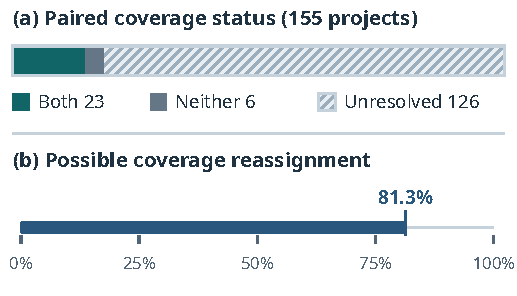
\includegraphics[width=\columnwidth]{consumer_holdout_evidence.pdf}
\caption{Paired consumer coverage evidence. The hatched segment shows unresolved pairs in the 155-application frame. The interval represents coverage reassignment compatible with the available evidence. All five-account tie choices give the same counts and bounds.}
\label{fig:consumer_holdout_evidence}
\end{figure}

We recorded all 155 projects and pinned 154 commits. Thirty projects entered the paired parser comparison and 25 yielded at least one corroborated path. The implementations agreed on 6,388 package locations in the compared projects. Arborist returned a virtual tree for 18 additional projects declined by the custom parser. Across the agreed paths, exact-version registry observations produced a usable maintainer list for 3,287 of 3,299 requested versions.

Figure~\ref{fig:consumer_holdout_evidence} shows the 23 documented common hits and six confirmed common negatives. Neither portfolio had an exclusive documented hit in any of the three comparisons. Each of the common hits had a witness from an account present in both portfolios. Twenty-nine outcomes were fully resolved, consisting of 23 common positives and six confirmed common negatives. The other 126 projects leave a full-reference turnover interval from 0 to 81.3\% and a net coverage interval from $-81.3$ to $+81.3$ percentage points. The identical-portfolio control gives zero turnover under all feasible assignments. The held-out study therefore cannot establish practical equivalence between the distinct portfolios. Access to applicable consumer trees is the primary measurement bottleneck in this frame.

\subsubsection{YunoHost comparison with broader lockfile support}
We applied the same frozen portfolios to a second frame of upstream applications from the YunoHost catalog. Requiring a root package manifest and excluding earlier repository keys and duplicate pinned commits yielded 215 projects. Lockfile intake identified 108 npm and 44 pnpm candidates. The other projects remain in the denominator.

For npm, we compare effective ranges from Arborist's virtual tree with checks against the committed dependency declarations, lockfile locations and pinned workspace manifests. The root walk follows verified links to local workspaces when those links are on a mandatory production path. Separate workspace importers are diagnostic because the catalog does not establish which importer is deployed. For pnpm lockfile format 9, we compare paths of up to three mandatory edges against the native offline listing. The depth limit lets those paths establish positive witnesses. A negative requires complete npm evidence within the supported root scope and an observed registry join for every retained witness.

We froze the comparison and the verification scope before acquiring the workspace manifests and observing the exact-version registry metadata used for scoring. A path's registry identity requires a canonical public npm tarball URL or an exact match between the lockfile's SHA-512 identifier and the registry response. We join maintainer associations after collection. Both frames measure committed dependency declarations and registry associations at the time of observation. The different intake and extraction rules limit direct comparisons between frames.
